\documentclass[conference]{IEEEtran}
\IEEEoverridecommandlockouts
% The preceding line is only needed to identify funding in the first footnote. If that is unneeded, please comment it out.
\usepackage{cite}
\usepackage{amsmath,amssymb,amsfonts}
\usepackage{algorithmic}
\usepackage{graphicx}
\usepackage{textcomp}
\usepackage{xcolor}

\usepackage{listings}
\usepackage{color}
\usepackage{stfloats}
\usepackage{subfigure}

\definecolor{dkgreen}{rgb}{0,0.6,0}
\definecolor{gray}{rgb}{0.5,0.5,0.5}
\definecolor{mauve}{rgb}{0.58,0,0.82}

\lstset{frame=tb,
  language=Python,
  aboveskip=3mm,
  belowskip=3mm,
  showstringspaces=false,
  columns=flexible,
  basicstyle={\small\ttfamily},
  numbers=none,
  numberstyle=\tiny\color{gray},
  keywordstyle=\color{blue},
  commentstyle=\color{dkgreen},
  stringstyle=\color{mauve},
  breaklines=true,
  tabsize=3
}

\def\BibTeX{{\rm B\kern-.05em{\sc i\kern-.025em b}\kern-.08em
    T\kern-.1667em\lower.7ex\hbox{E}\kern-.125emX}}
\begin{document}


\title{Project A:Visual Interpretation of Convolutional Neural Networks}

\begin{abstract}
This paper is a report for Project A of ECE1512 2022W, University of Toronto. In the paper, we described four assigned tasks with detail, including CNN construction and training, statistic assessment, XAI based interpretation and Quantitative evaluation. For the attribution methods, we choose Grad-CAM, Grad-CAM++ and Ablation-CAM as a group of two, and we reviewed their paper and implemented corresponding functions. Moreover, we tried to analyze the performance of the XAI methods based on quantitative evaluation and gave our explanations towards the experiment.
\end{abstract}

\section{Task 1: 1-Dimensional digit classification}
\subsection{Question 1}
\begin{lstlisting}
    weight_decay = 5e-4
    model = Sequential()
    #Your code starts from here 
    model.add(Input(shape=(40,1)))
    model.add(Conv1D(25, kernel_size=5, padding='same', activation='relu', kernel_regularizer=regularizers.l2(weight_decay)))
    model.add(Conv1D(25, kernel_size=3, padding='same', activation='relu', kernel_regularizer=regularizers.l2(weight_decay)))
    model.add(Conv1D(25, kernel_size=3, padding='same', activation='relu', kernel_regularizer=regularizers.l2(weight_decay)))

    model.add(Flatten())
    model.add(Dense(10, activation='softmax', kernel_initializer=keras.initializers.RandomNormal(mean=0.0, stddev=0.5),
                    bias_initializer=keras.initializers.Zeros(), kernel_regularizer=regularizers.l2(weight_decay)))

    model.summary()
\end{lstlisting}
In this question, we build a ConvNet. It includes three convolutional layer, one flatten layer and one dense layer.
The network is listed as Fig. 1:
\begin{figure}[h] 
    \centering %图片居中
    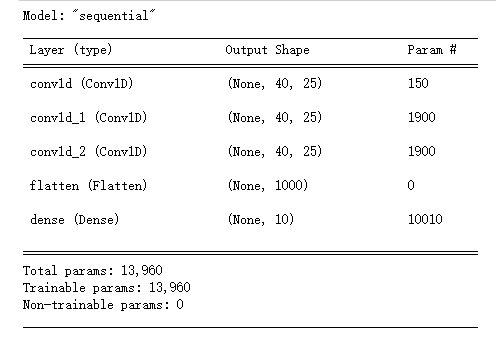
\includegraphics[width=0.3\textwidth]{T1Q1.png} %插入图片,[]中设置图片大小,{}中是图片文件名
    \caption{Task1-Question1: ConvNet Model} %最终文档中希望显示的图片标题
    \label{Fig.t1q1} %用于文内引用的标签
\end{figure}
\subsection{Question 2}
In this section, we apply the model in question 1 to the MNIST1D dataset. The code is listed as followed:
\begin{lstlisting}
    model.compile(loss=keras.losses.categorical_crossentropy,
              optimizer=tensorflow.keras.optimizers.SGD(),
              metrics=['accuracy'])

    def lr_scheduler(epoch):
        base_ep = 15
        return 1e-3 * (.5 ** (epoch // base_ep))
    lr_reduce_cb = keras.callbacks.LearningRateScheduler(lr_scheduler)
    tensorboard_cb = keras.callbacks.TensorBoard(log_dir='log2', write_graph=True)
    early_stopping_cb = keras.callbacks.EarlyStopping(patience=8, min_delta=0.)

    # X = tensorflow.expand_dims(dataset['x'],axis=2)
    train_x=dataset['x']
    train_y=dataset['y']
    train_x=train_x.reshape(4000,40,1)
    train_y=tensorflow.keras.utils.to_categorical(train_y, num_classes=10)

    # print(X.shape)
    history=model.fit(x=train_x,y=train_y,epochs=200,
    #                     steps_per_epoch=len(X) // 32,
                        callbacks=[tensorboard_cb],                  
                        shuffle = True,
                        verbose=1)
    model.save('MNIST1D.h5')
\end{lstlisting}
Here, we use the tensorboard to record the training procedure.First of all, we compile this model, set the loss function to cross-entropy, set the optimizer to Stochastic Gradient Descent and the metrics to accuracy. 
Then we define the LearningRateScheduler, the TensorBoard, the EarlyStopping for later use.
After that, we handle the train data for training.
At last, we will fit the data and tensorboard into the model for training and save the model into disk.
The training result is shown as followed\ref{Fig.t1q2}:
\begin{figure}[h] 
    \centering %图片居中
    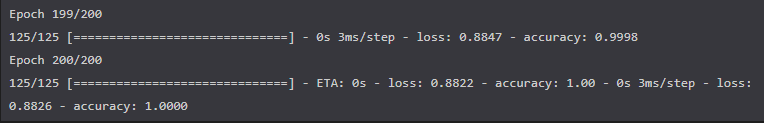
\includegraphics[width=0.5\textwidth]{T1Q2.png} %插入图片,[]中设置图片大小,{}中是图片文件名
    \caption{Task1-Question2: Training Process Log} %最终文档中希望显示的图片标题
    \label{Fig.t1q2} %用于文内引用的标签
\end{figure}
\subsection{Question 3}
\subsubsection{SubQuestion a}
This is the code for loss and accuracy curve.
\begin{lstlisting}
    train_acc = history.history['accuracy']
    train_loss = history.history['loss']
    plt.plot(train_acc)
    plt.figure()
    plt.plot(train_loss)
\end{lstlisting}
In the code, we used the training history defined in the previous code to do the plot.
The plot of loss curve\ref{Fig.t1q3a1} and plot for accuracy curve\ref{Fig.t1q3a2} are shown below:
\begin{figure}[H] 
    \centering %图片居中
    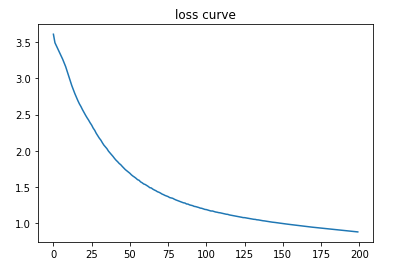
\includegraphics[width=0.3\textwidth]{T1Q3-b.png} %插入图片,[]中设置图片大小,{}中是图片文件名
    \caption{Task1-Question3a-1: Loss Curve of 1-D CNN} %最终文档中希望显示的图片标题
    \label{Fig.t1q3a1} %用于文内引用的标签
\end{figure}
\begin{figure}[h] 
    \centering %图片居中
    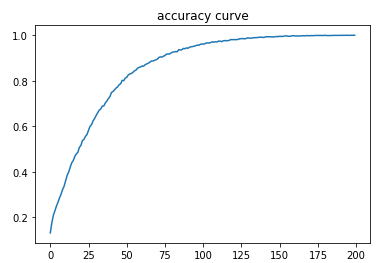
\includegraphics[width=0.3\textwidth]{T1Q3-a.png} %插入图片,[]中设置图片大小,{}中是图片文件名
    \caption{Task1-Question3a-2: Accuracy Curve of 1-D CNN} %最终文档中希望显示的图片标题
    \label{Fig.t1q3a2} %用于文内引用的标签
\end{figure}
\subsubsection{SubQuestion b}
This part talks about overall classification accuracy on the test set.
\begin{lstlisting}
    # Use Scikit-learn to calculate stats
    from sklearn.metrics import accuracy_score, precision_score, recall_score,f1_score
    from sklearn.metrics import classification_report

    # Q3.b get the prediction from the test set
    x_test = dataset['x_test']
    y_test = dataset['y_test']
    x_test=x_test.reshape(1000,40,1)
    # predict_classes removed in tf 2.6.0
    y_pred = model.predict(x_test)
    y_predicted = np.argmax(y_pred,axis=1)
    print('Overall classification accuracy for all classes:'+str(np.sum(y_predicted==y_test)/y_test.shape[0]))
\end{lstlisting}
We read the test set, fit the model on the set and calculate the accuracy by deciding the max prediction in every class and compare them with the ground truth. The result is 0.919\ref{Fig.t1q3b}.

\begin{figure}[H] 
    \centering %图片居中
    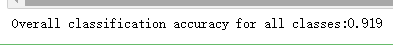
\includegraphics[width=0.7\textwidth]{T1Q3b.png} %插入图片,[]中设置图片大小,{}中是图片文件名
    \caption{Task1-Question3b: overall accuracy} %最终文档中希望显示的图片标题
    \label{Fig.t1q3b} %用于文内引用的标签
\end{figure}
\subsubsection{SubQuestion c}
In this part, we calculated the class-wise accuracy for all classes.This is our code:
\begin{lstlisting}
    # Q3.c class-wise classification
for i in range(10):
    true_i=np.where(y_test==i)[0]
    res=0
    for j in true_i:
        if y_predicted[j]==i:
            res=res+1
    print('class '+str(i)+' accuracy:'+str(res/true_i.shape[0]))
#     pred_i=np.where(y_predicted[true_i]==i)[0]
#     print('class '+str(i)+' accuracy:'+str(pred_i.shape[0]/true_i.shape[0]))
\end{lstlisting}
We find out the lines which belongs to class i and find the ones which is correct in these lines to calculate the accuracy.
The result is shown below\ref{Fig.t1q3c}:
\begin{figure}[H] 
    \centering %图片居中
    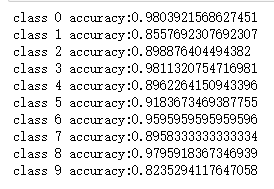
\includegraphics[width=0.7\textwidth]{T1Q3c.png} %插入图片,[]中设置图片大小,{}中是图片文件名
    \caption{Task1-Question3b: class-wise accuracy} %最终文档中希望显示的图片标题
    \label{Fig.t1q3c} %用于文内引用的标签
\end{figure}
\subsubsection{SubQuestion d}
In this part, we will plot the ROC and AUC curves for each class.
Here is the code:
\begin{lstlisting}
    # Q3.d ROC and AUC curve for every class
    from sklearn.metrics import roc_curve
    from sklearn.metrics import auc
    # print(dataset['y_test'].shape)
    real_y=np.zeros((dataset['y_test'].size,10))
    for i in range(y_test.size):
        real_y[i,y_test[i]]=1
    for i in range(10):
        FPR, TPR, thresholds_keras = roc_curve(real_y[:,i], y_pred[:,i])   
        AUC = auc(FPR, TPR)
        print("AUC : ", AUC)
        plt.figure()
        plt.plot([0, 1], [0, 1], 'k--')
        plt.plot(FPR, TPR, label='S3< val (AUC = {:.3f})'.format(AUC))
        plt.xlabel('False positive rate')
        plt.ylabel('True positive rate')
        plt.title('ROC curve for class '+str(i))
        plt.legend(loc='best')
        plt.show()   
\end{lstlisting}
In the code, we first reshape the test set to 2D set. Then we apply the test set and prediction set to roc_curve.
Then we will calculate the auc number and plot the curve.The AUC and ROC curve is listed below:
This is class 0\ref{Fig.ROC0}:
\begin{figure}[H] 
    \centering %图片居中
    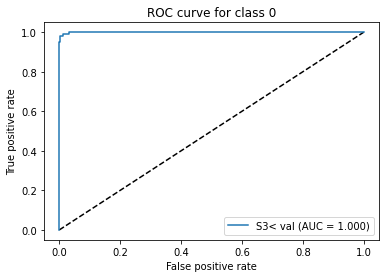
\includegraphics[width=0.7\textwidth]{ROC0.png} %插入图片,[]中设置图片大小,{}中是图片文件名
    \caption{AUC for class 0:  0.9995087121708371} %最终文档中希望显示的图片标题
    \label{Fig.ROC0} %用于文内引用的标签
\end{figure}
This is class 1\ref{Fig.ROC1}:
\begin{figure}[H] 
    \centering %图片居中
    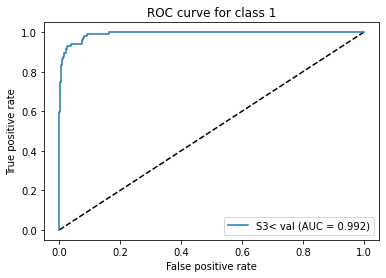
\includegraphics[width=0.7\textwidth]{ROC1.png} %插入图片,[]中设置图片大小,{}中是图片文件名
    \caption{AUC for class 1:  0.991919213598901} %最终文档中希望显示的图片标题
    \label{Fig.ROC1} %用于文内引用的标签
\end{figure}
This is class 2\ref{Fig.ROC2}:
\begin{figure}[H] 
    \centering %图片居中
    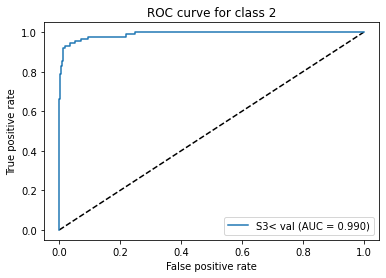
\includegraphics[width=0.7\textwidth]{ROC2.png} %插入图片,[]中设置图片大小,{}中是图片文件名
    \caption{AUC for class 2:  0.9901700810320798} %最终文档中希望显示的图片标题
    \label{Fig.ROC2} %用于文内引用的标签
\end{figure}
This is class 3\ref{Fig.ROC3}:
\begin{figure}[H] 
    \centering %图片居中
    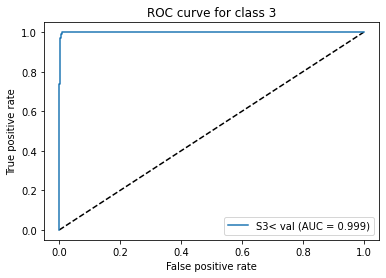
\includegraphics[width=0.7\textwidth]{ROC3.png} %插入图片,[]中设置图片大小,{}中是图片文件名
    \caption{AUC for class 3:  0.9992718753957199} %最终文档中希望显示的图片标题
    \label{Fig.ROC3} %用于文内引用的标签
\end{figure}
This is class 4\ref{Fig.ROC4}:
\begin{figure}[H] 
    \centering %图片居中
    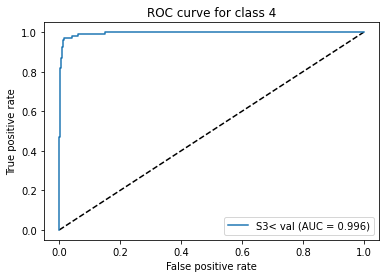
\includegraphics[width=0.7\textwidth]{ROC4.png} %插入图片,[]中设置图片大小,{}中是图片文件名
    \caption{AUC for class 4:  0.9955784897218353} %最终文档中希望显示的图片标题
    \label{Fig.ROC4} %用于文内引用的标签
\end{figure}
This is class 5\ref{Fig.ROC5}:
\begin{figure}[H] 
    \centering %图片居中
    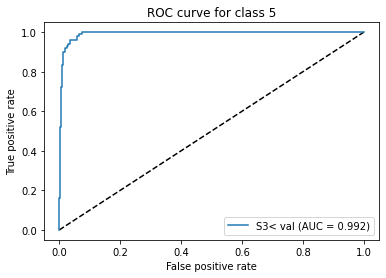
\includegraphics[width=0.7\textwidth]{ROC5.png} %插入图片,[]中设置图片大小,{}中是图片文件名
    \caption{AUC for class 5:  0.9922620933073896} %最终文档中希望显示的图片标题
    \label{Fig.ROC5} %用于文内引用的标签
\end{figure}
This is class 6\ref{Fig.ROC6}:
\begin{figure}[H] 
    \centering %图片居中
    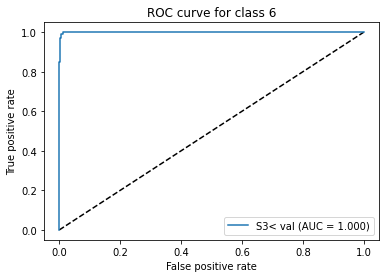
\includegraphics[width=0.7\textwidth]{ROC6.png} %插入图片,[]中设置图片大小,{}中是图片文件名
    \caption{AUC for class 6:  0.9995851971434657} %最终文档中希望显示的图片标题
    \label{Fig.ROC6} %用于文内引用的标签
\end{figure}
This is class 7\ref{Fig.ROC7}:
\begin{figure}[H] 
    \centering %图片居中
    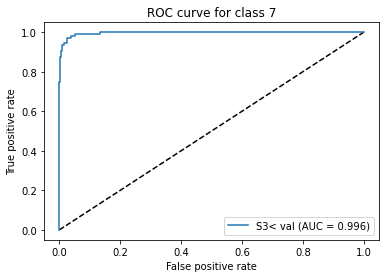
\includegraphics[width=0.7\textwidth]{ROC7.png} %插入图片,[]中设置图片大小,{}中是图片文件名
    \caption{AUC for class 7:  0.9961167957227138} %最终文档中希望显示的图片标题
    \label{Fig.ROC7} %用于文内引用的标签
\end{figure}
This is class 8\ref{Fig.ROC8}:
\begin{figure}[H] 
    \centering %图片居中
    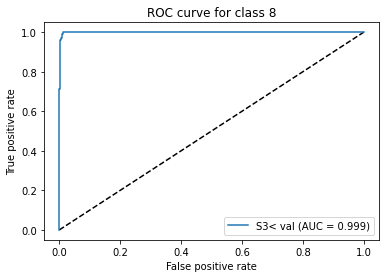
\includegraphics[width=0.7\textwidth]{ROC8.png} %插入图片,[]中设置图片大小,{}中是图片文件名
    \caption{AUC for class 8:  0.9992420471514548} %最终文档中希望显示的图片标题
    \label{Fig.ROC8} %用于文内引用的标签
\end{figure}
This is class 9\ref{Fig.ROC9}:
\begin{figure}[H] 
    \centering %图片居中
    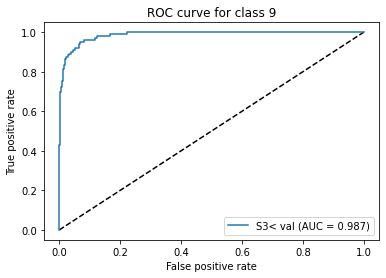
\includegraphics[width=0.7\textwidth]{ROC9.png} %插入图片,[]中设置图片大小,{}中是图片文件名
    \caption{AUC for class 9:  0.986538713480938} %最终文档中希望显示的图片标题
    \label{Fig.ROC9} %用于文内引用的标签
\end{figure}
\subsubsection{SubQuestion e}
This is the code for normalized confusion matrix.
\begin{lstlisting}
    from sklearn.metrics import confusion_matrix
    cm=confusion_matrix(list(y_test),list(y_predicted))
    cm_normalized = cm.astype('float') / cm.sum(axis=1)[:, np.newaxis]
    fig, ax = plt.subplots()
    im = ax.imshow(cm, interpolation='nearest', cmap=plt.cm.Blues)
    ax.figure.colorbar(im, ax=ax)
    classes=[0,1,2,3,4,5,6,7,8,9]
    # print(classes)
    # We want to show all ticks...
    ax.set(xticks=np.arange(cm_normalized.shape[1]),
        yticks=np.arange(cm_normalized.shape[0]),
        # ... and label them with the respective list entries
        xticklabels=classes, yticklabels=classes,
        ylabel='True label',
        xlabel='Predicted label')
    plt.setp(ax.get_xticklabels(),  ha="right",
                rotation_mode="anchor")
    thresh = cm_normalized.max() / 2.
    for i in range(cm_normalized.shape[0]):
        for j in range(cm_normalized.shape[1]):
            ax.text(j, i, format(cm_normalized[i, j], '.2f'),
                    ha="center", va="center",
                    color="white" if cm_normalized[i, j] > thresh else "black")
    fig.tight_layout()
\end{lstlisting}
The result plot is listed in Fig.\ref{Fig.t1q3e}.
\begin{figure}[H] 
    \centering %图片居中
    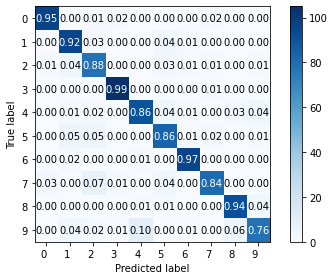
\includegraphics[width=0.7\textwidth]{T1Q3e.png} %插入图片,[]中设置图片大小,{}中是图片文件名
    \caption{normalized confusion matrix plot} %最终文档中希望显示的图片标题
    \label{Fig.t1q3e} %用于文内引用的标签
\end{figure}
\subsubsection{SubQuestion f}
This is the code for calculating Precision, Recall, and F-1 score on the test set.
\begin{lstlisting}
    # Q3.f
    print(classification_report(y_true=y_test,y_pred=y_predicted))
\end{lstlisting}
This is the result for the plot\ref{Fig.t1q3f}:
\begin{figure}[H] 
    \centering %图片居中
    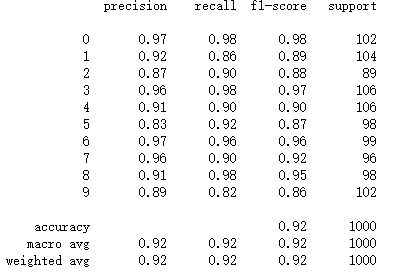
\includegraphics[width=0.7\textwidth]{T1Q3f.png} %插入图片,[]中设置图片大小,{}中是图片文件名
    \caption{Precision,Recall and F-1 score} %最终文档中希望显示的图片标题
    \label{Fig.t1q3f} %用于文内引用的标签
\end{figure}
\subsection{Question 4}
To do this question, we did some coding in our program, the codes are listed below:

Success Examples:
\begin{lstlisting}
    index 10 true class: 0 predicted class: 0
    index 412 true class: 1 predicted class: 1
    index 729 true class: 2 predicted class: 2
    \end{lstlisting}
Failure Examples:
\begin{lstlisting}
    index 236 true class: 0 predicted class: 7
    index 6 true class: 1 predicted class: 2
    index 25 true class: 1 predicted class: 4
\end{lstlisting}
The concrete Success/Failure cases are recorded in 'MNIST1D.ipynb', if you want to refer to more examples.
The most misclassification lies in class 1 and 4.
The reason for that is TODOOO: analyze
挑几个正确与错误的例子,评价一下,哪两个类错误最多
\section{Task 2: CNN interprectation}

This section introduces our interpretation of 1-D CNN model based on MNIST-1D dataset using 3 different attribution methods, including our literature review, discussion and implementation of the XAI attribute algorithms.

\subsection{Grad-CAM}
In the previous study, researchers introduced CAM to explain the CNN. However, CAM requires to modify the structure of original training models. It limits the usage of CAM greatly, because the cost of retraining the model is quite high for the published model. It is almost impossible to retrain them.
To solve this problem, Grad-CAM was proposed, which is similar to CAM. It also gets the weight of every feature maps and calculate the results accordingly. The difference lies in the calculation of weights. CAM replaced full-connection layer with GAP layer and retrain this whole model. In contrast to that, Grad-CAM put forward a new way to do it.
It calculates the weight by averaging the gradients which is equivalent to the CAM. It makes CAM applicable to all the existing models.\par

The core algorithm of Grad-CAM is based on CAM which proposed: class c gets the final classification score $Y_{c}$ with a linear combination of its global average pooled last convolutional layer feature maps $A_{}k$\ref{Grad-CAM-1}.
\begin{equation}
\begin{aligned}
    Y^{c}=\Sigma_{k}w_{k}^{c}\Sigma_{i}\Sigma_{j}A_{ij}^{k})
    \label{Grad-CAM-1}
\end{aligned}
\end{equation}
So, first, it defines the weight of feature map $k$ to class $c$ as $\alpha_{k}^{c}$, and it calculates the weight using the global gradients\ref{Grad-CAM_alpha}:
\begin{equation}
    \begin{aligned}
        \alpha_{k}^{c}=\frac{1}{Z}*\Sigma_{i}\Sigma_{j}\frac{\partial y^{c}}{\partial A_{ij}^{k}}
        \label{Grad-CAM_alpha}
    \end{aligned}
  \end{equation}
  In which, $y_{c}$ is the gradient of the score for class c, $A_{k}$ is the feature map activation.$\frac{\partial y^{c}}{\partial A_{ij}^{k}}$ is the gradient achieved by backpropagating. $\frac{1}{Z}$ is global averaging.
  After calculating the $\alpha_{k}^{c}$, the algorithm computed the weighted combination of forward activation maps, followed by a ReLU function:
  
  \begin{equation}
  \begin{aligned}
      L_{Grad-CAM}^{c}=ReLU(\Sigma_{k}\alpha_{k}^{c}A^{k})
      \label{Grad-CAM_weight}
  \end{aligned}
\end{equation}
The advantages for Grad-CAM is quite obvious: First, compared with CAM, it does not need to change the model and retrain it which costs a lot of time and money. 
The novelty is the usage of propagation and gradients to compute the weights of feature maps.It makes the visualization of published models possible. Second is that the algorithm is quite easy to code and maintain.\par
The disadvantages for Grad-CAM is that: it considers the global features for all classes. As a result, Grad-CAM cannot localize the targets when faced with many targets of the same class. If there are many objects of the same class in an image, it cannot localize the targets well or it can only locate part of them.

\subsection{Grad-CAM++}
Grad-CAM++ is an algorithm based on Grad-CAM, aiming to get a better explanation for CNN models. It improves the performance of Grad-CAM when facing targets of the same class, and helps to better localize the targets.\par
It introduced a weighted combination of gradients of the output in the pixel level, which provides a measure of importance of every pixels to the feature maps.
It introduced a closed-form solution for the pixels weights, thus making the improvement of explanation possible. \par
The core algorithm is shown below:
First, as we have introduced above, class c gets the final classification score $Y_{c}$ with a linear combination of its global average pooled last convolutional layer feature maps $A_{}k$ in equation\ref{Grad-CAM_alpha}.
Grad-CAM calculates the weight $w_{k}^{c}$ with equation\ref{Grad-CAM_weight}.  To improve the performance, Grad-CAM++ changed this equation.
Combine the equation\ref{Grad-CAM_alpha} and \ref{Grad-CAM-1} together, we will get the equation\ref{Grad-CAMPP-1}:
\begin{equation}
    \begin{aligned}
        Y^{c}=\Sigma_{k}[\Sigma_{i}\Sigma_{j}(\Sigma_{a}\Sigma_{b}\alpha_{ab}^{kc}·relu(\frac{\partial Y_{c}}{\partial A_{ab}^{k}}))A_{ij}^{k}]
        \label{Grad-CAMPP-1}
    \end{aligned}
\end{equation}
Take partial derivative w.r.t. $A_{ij}^{k}$ on both sides:
\begin{equation}
\begin{aligned}
    \frac{\partial Y_{c}}{\partial A_{ij}^{k}}=\Sigma_{a}\Sigma{b}\alpha_{ab}^{kc}·\frac{\partial Y_{c}}{\partial A_{ij}^{k}}+\Sigma_{a}\Sigma{b}\alpha_{ab}^{k}\{\alpha_{ab}^{kc}·\frac{\partial^{2} Y_{c}}{(\partial A_{ij}^{k})^_{2}}\}
    \label{Grad-CAMPP-2}
\end{aligned}
\end{equation}
Take a further partial derivative w.r.t. $A_{ij}^{k}$ on both sides:
\begin{equation}
    \begin{aligned}
        \frac{\partial^{2} Y_{c}}{(\partial A_{ij}^{k})^_{2}}=2·\alpha_{ab}^{kc}·\frac{\partial^{2} Y_{c}}{(\partial A_{ij}^{k})^_{2}}+\Sigma_{a}\Sigma{b}\alpha_{ab}^{k}\{\alpha_{ab}^{kc}·\frac{\partial^{3} Y_{c}}{(\partial A_{ij}^{k})^_{3}}\}
        \label{Grad-CAMPP-3}
    \end{aligned}
    \end{equation}
Rearrage equation\ref{Grad-CAMPP-3}, we get:
    \begin{equation}
        \begin{aligned}
            \alpha_{ab}^{kc}=\frac{\frac{\partial^{2} Y_{c}}{(\partial A_{ij}^{k})^_{2}}}{2\frac{\partial^{2} Y_{c}}{(\partial A_{ij}^{k})^_{2}}+\Sigma_{a}\Sigma{b}\alpha_{ab}^{k}\{\frac{\partial^{3} Y_{c}}{(\partial A_{ij}^{k})^_{3}}\}}
            \label{Grad-CAMPP-4}
        \end{aligned}
        \end{equation}
So, we are able to get weight $w_{k}$ with:
\begin{equation}
    \begin{aligned}
        w_{k}^{c}=\Sigma_{i}\Sigma_{j}\alpha_{ij}^{kc}·relu(\frac{\partial Y_{c}}{\partial A_{ij}^{k}})
        \label{Grad-CAMPP-5}
    \end{aligned}
    \end{equation}
Applying equation\ref{Grad-CAMPP-5} to \ref{Grad-CAM_weight}, we will get final results.
There are many advantages for Grad-CAM++: First, it clearly improved the performance of Grad-CAM when facing with many objects of the same class in an image. It helps us to localize the objects more accurately. 
Second is that it only adds tow partial derivative to the computation, and it uses backpropagation only once. So it does not increase the computation time a lot.\par
However, it still remains to be revised in some aspects: First, although it improved the performance of Grad-CAM in some degrees, its performance is far from perfect. The same problem remains and connot be solved completelly. 
Second, from my perspective, ignoring the relu function in the alpha calculation will decrease the precision.\par
Our implementation code is as followed:
\begin{lstlisting}
    ef grad_cam_plus_plus(input_model, image, layer_name, class_index=None):
    # if class_index is None:
    #     class_index=np.argmax(input_model.predict(np.array([image])), axis=-1)[0]
    """GradCAM method for visualizing input saliency."""
    # cls = np.argmax(input_model.predict(image))
    y_c = input_model.output
    conv_output = input_model.get_layer(layer_name).output
    feedforward1 = keras.models.Model([input_model.input], [conv_output, y_c])
    # with tf.GradientTape() as tape1:
    #     with tf.GradientTape() as tape2:
    #         with tf.GradientTape() as tape3:
    #             ff_results = feedforward1([image])
    #             all_fmap_masks, predictions = ff_results[0], ff_results[-1]
    if class_index==None:
        cls=np.argmax(input_model.predict(image))
    else:
        cls=class_index
    #             loss = predictions[:, cls]
    #         grads_val = tape3.gradient(loss, all_fmap_masks)
    #     grads_val2 = tape2.gradient(grads_val, all_fmap_masks)
    # grads_val3 = tape1.gradient(grads_val2, all_fmap_masks)
    with tf.GradientTape() as tape:
        ff_results=feedforward1([image])
        all_fmap_masks, predictions = ff_results[0], ff_results[-1]
        loss = predictions[:, cls]
    grads_val = tape.gradient(loss, all_fmap_masks)
    grads_val2=grads_val**2
    grads_val3=grads_val2*grads_val
    if len(image.shape) == 3:
        axis = (0, 1)
    elif len(image.shape) == 4:
        axis = (0, 1, 2)
    alpha_div=(2.0 * grads_val2 + grads_val3 * np.sum(all_fmap_masks, axis))
    alpha_div = np.where(alpha_div != 0.0, alpha_div, 0)
    alpha = grads_val2 / alpha_div
    weights = np.maximum(grads_val, 0.0) * alpha
    weights = np.sum(weights, axis=axis)
    # weights = np.mean(grads_val, axis=axis)
    cam = np.dot(all_fmap_masks[0], weights)
    # print (cam)
    H, W = image.shape[1:3]
    cam = np.maximum(cam, 0)
    # cam = resize(cam, (H, W))
    cam = zoom(cam, H / cam.shape[0])
    # cam = np.maximum(cam, 0)
    cam = cam / cam.max()
    return cam
\end{lstlisting}
\subsection{Ablation-CAM}

The Ablation-CAM creatively uses ablation analysis to determine the importance of individual feature map units for different classes. It proposes a novel “gradient-free” visualization approach which avoids use of gradients and at the same time, produce high quality class-discriminative localization maps.\par

The core algorithm of Ablation-CAM is not complex: it uses the value of slope to describe the effect of ablation of individual unit $k$ by the following formula:

$$slope = \frac{y^c-y^c_k}{||A_k||}$$

In the formula, $y^c$ stands for activation score of class c, which represent the entire class activation status. $y^c_k$ indicates the value of the function for absence of unit $k$, where $A_k$ is the baseline. Those concepts lead us to ablation study, which is the basic principle of the method.\par
Ablation study is a method to distribute the influencing importance of different factors by controlling the variable while switching the combination of potential factors, and also their standalone. For example, if we'd like to know whether $A$ or $B$ component of medicine could improve the effect of an old medicine $C$. We could compare $C+A$, $C+B$ and also $C+A+B$ with the baseline of $C$. We could know if the A or B or they together are able to improve the effect. In the instance of Ablation-CAM, different unit $k$ is the "component", and the whole feature map is so-called baseline, $A_k$. Thus, using slope described in the previous formula could represent the importance of a single unit to the feature map.\par
However practically, norm $||A_k||$ is hard to compute due to its large size and hence the slope could be approximately presented by the following formula, assuming a very small value.

$$w^c_k = \frac{y^c-y^c_k}{y^c}$$

As the algorithm, Ablation-CAM can then be obtained as weighted linear combination of activation maps and corresponding weights from the formula above, which is somehow similar to that of Grad-CAM.

$$L^C_{Ablation-CAM}=ReLU(\sum_k {w^c_k}{A_k})$$

There are a number of advantages and features of Ablation-CAM. Firstly, a significant contribution and novelty of the Ablation-CAM is the ablation analysis it used to decide the weights of feature map units. Secondly, it could produce a coarse localization map highlighting the regions in the image for prediction. Thirdly, compare to other CAM methods, this approach works essentially better when it is full connected to obtain the result, which is known as final linear classifier, and have as good performance as other gradient-based CAM methods when evaluating other CNNs. Last but not the least, the approach introduce a gradient-free principle which avoids use of gradient as Grad-CAM does and produce a high-quality class-wise localization maps, which helps it to adapt into any CNN based architecture.\par
However, the approach have some limitations as well. First of all, the computational time required to generate a single Ablation-CAM is much grater than the required for Grad-CAM, as it has to iterate over each feature map to ablate it and check the drop in class activation score correspondingly. 
On the hand, the Ablation-CAM only benefits the interpretation where last convolutional layer is not followed immediately by decision nodes, yet show the same performance statistically as other CAM methods.\par

Our implementation code is as followed.

\begin{lstlisting}
def extract_feature_map(img, model, class_index=None, layer_name="conv1d_2"):
    # Get gradients for the class on the last conv layer
    gradModel = tf.keras.models.Model([model.inputs],[model.get_layer(layer_name).output, model.output])
    print("gradModel = ")
    print(gradModel)
    # Get Activation Map on the last conv layer
    with tf.GradientTape() as tape:
        # Get Prediction on the last conv layer
        convOutputs, predictions = gradModel(np.array([img]))
        output = convOutputs[0]
        print("#prediction#")
        print(predictions)
        print("OUTPUT")
        print(output)
    
    if class_index is None:
        class_index = np.argmax(model.predict(np.array([img])), axis = -1)[0]
        y_class = np.max(model.predict(np.array([img])))
    else:
        y_class = model.predict(np.array([img]))[0][class_index]

    # Get Weights on the layer
    weights = np.zeros(model.get_layer(layer_name).get_weights()[1].shape)
    # Get Weights for the maps
    allWeights = model.get_layer(layer_name).get_weights().copy()
    zeroWeight = allWeights[0][:,:,:,0]*0
    localWeight = [np.zeros(allWeights[0].shape)]
    localWeight.append(np.zeros(allWeights[1].shape))

    for i in range(weights.shape[0]):
        localWeight[0] = allWeights[0].copy()
        localWeight[0][:,:,:,i] = zeroWeight
        model.get_layer(layer_name).set_weights(localWeight)
        y_pred = model.predict(np.array([img]))[0][class_index]
        weights[i] = (y_class - y_pred)/y_class # Simplified Formula
        model.get_layer(layer_name).set_weights(allWeights)

    outputMean = np.mean([output[:,:,i] for i in range(output.shape[2])], axis = 0)
    outputMean = np.maximum(outputMean, 0.0)
    outMeanMask = np.zeros(output.shape[0:2], dtype = np.float32)
    for i in range(output.shape[0]):
        for j in range(output.shape[1]):
            if outputMean[i][j] < np.mean(outputMean[:,:]):
                outMeanMask[i][j] = 255
            else:
                outMeanMask[i][j] = 0
    return weights, output, outputMean, outMeanMask

def ablation_cam(weights, output):
    ablationMap = weights * output
    ablationCam = np.sum(ablationMap, axis=(2))

    ablationMask = np.zeros(ablationMap.shape[0:2], dtype = np.float32)
    for i in range(ablationMap.shape[0]):
        for j in range(ablationMap.shape[1]):
            if ablationCam[i][j] < np.mean(ablationCam[:,:]):
                ablationMask[i][j] = 255
            else:
                ablationMask[i][j] = 0
    
    return ablationCam, ablationMask
\end{lstlisting}

\section{Task 3: Biomedical image classification and interpretation}
\subsection{Question 1}
\subsubsection{Overall classification accuracy}
Here we calculate the overall classification accuracy, here is the code:
\begin{lstlisting}
    from sklearn.metrics import accuracy_score, precision_score, recall_score,f1_score
    from sklearn.metrics import classification_report
    from sklearn.metrics import roc_curve, auc
    from sklearn.metrics import confusion_matrix

    test_generator.reset()
    y_test=test_generator.classes
    y_pred=model.predict(test_generator)
    y_predicted=np.argmax(y_pred, axis=1)
    print('Overall classification accuracy for all classes:'+str(np.sum(y_predicted==y_test)/y_test.shape[0]))
\end{lstlisting}
The result is 0.8306451612903226, as is shown in Fig\ref{Fig.t3q1}:
\begin{figure}[H] 
    \centering %图片居中
    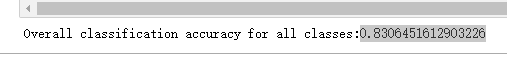
\includegraphics[width=0.7\textwidth]{T3Q1a.png} %插入图片,[]中设置图片大小,{}中是图片文件名
    \caption{Overall classification accuracy} %最终文档中希望显示的图片标题
    \label{Fig.t3q1} %用于文内引用的标签
\end{figure}
\subsubsection{class-wise classification accuracy}
In this part, we discuss the classification accuracy for every class.Here is the code:
\begin{lstlisting}
    for i in range(8):
    true_i=np.where(y_test==i)[0]
    res=0
    for j in true_i:
        if y_predicted[j]==i:
            res=res+1
    print('class '+str(i)+' accuracy:'+str(res/true_i.shape[0]))
\end{lstlisting}
The results are shown in Fig\ref{Fig.t3q2}:
\begin{figure}[H] 
    \centering %图片居中
    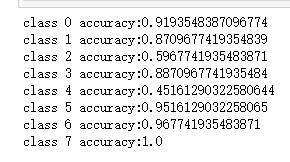
\includegraphics[width=0.7\textwidth]{T3Q1b.png} %插入图片,[]中设置图片大小,{}中是图片文件名
    \caption{class-wise classification accuracy} %最终文档中希望显示的图片标题
    \label{Fig.t3q2} %用于文内引用的标签
\end{figure}
\subsubsection{AUC-ROC curve}
In this part, we discuss the AUC and ROC curve.Here is the code:
\begin{lstlisting}
    real_y=np.zeros((y_test.size,8))
    for i in range(y_test.size):
        real_y[i,y_test[i]]=1
    for i in range(8):
        FPR, TPR, thresholds_keras = roc_curve(real_y[:,i], y_pred[:,i]) 
        AUC = auc(FPR, TPR)  
        print("AUC for class "+str(i)+": ", AUC)
        plt.figure()
        plt.plot([0, 1], [0, 1], 'k--')
        plt.plot(FPR, TPR, label='S3< val (AUC = {:.3f})'.format(AUC))
        plt.xlabel('False positive rate')
        plt.ylabel('True positive rate')
        plt.title('ROC curve for class '+str(i))
        plt.legend(loc='best')
        plt.show()    
\end{lstlisting}
The plots are shown below:
\begin{figure}[H] 
    \centering %图片居中
    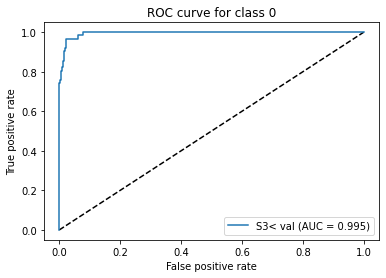
\includegraphics[width=0.7\textwidth]{3ROC0.png} %插入图片,[]中设置图片大小,{}中是图片文件名
    \caption{AUC for class 0:  0.9948714137059611} %最终文档中希望显示的图片标题
    \label{Fig.3ROC0} %用于文内引用的标签
\end{figure}
This is class 1\ref{Fig.ROC1}:
\begin{figure}[H] 
    \centering %图片居中
    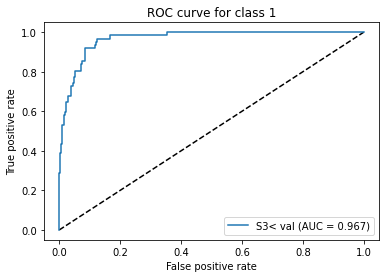
\includegraphics[width=0.7\textwidth]{3ROC1.png} %插入图片,[]中设置图片大小,{}中是图片文件名
    \caption{AUC for class 1:  0.9665526980823547} %最终文档中希望显示的图片标题
    \label{Fig.3ROC1} %用于文内引用的标签
\end{figure}
This is class 2\ref{Fig.ROC2}:
\begin{figure}[H] 
    \centering %图片居中
    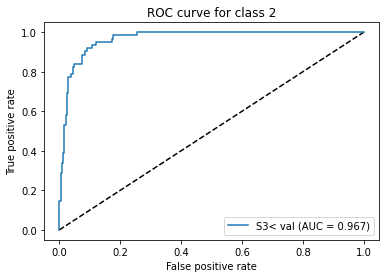
\includegraphics[width=0.7\textwidth]{3ROC2.png} %插入图片,[]中设置图片大小,{}中是图片文件名
    \caption{AUC for class 2:  0.9670358257767206} %最终文档中希望显示的图片标题
    \label{Fig.3ROC2} %用于文内引用的标签
\end{figure}
This is class 3\ref{Fig.ROC3}:
\begin{figure}[H] 
    \centering %图片居中
    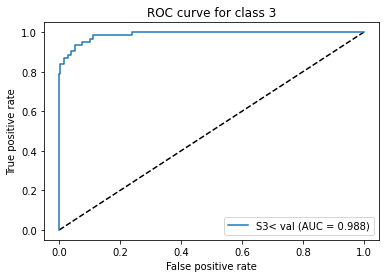
\includegraphics[width=0.7\textwidth]{3ROC3.png} %插入图片,[]中设置图片大小,{}中是图片文件名
    \caption{AUC for class 3:  0.9882562806600268} %最终文档中希望显示的图片标题
    \label{Fig.3ROC3} %用于文内引用的标签
\end{figure}
This is class 4\ref{Fig.ROC4}:
\begin{figure}[H] 
    \centering %图片居中
    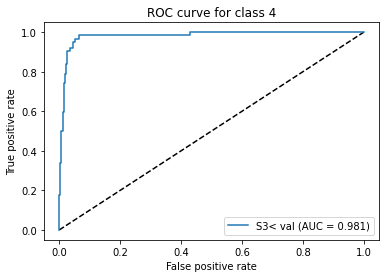
\includegraphics[width=0.7\textwidth]{3ROC4.png} %插入图片,[]中设置图片大小,{}中是图片文件名
    \caption{AUC for class 4:  0.9813066745949159} %最终文档中希望显示的图片标题
    \label{Fig.3ROC4} %用于文内引用的标签
\end{figure}
This is class 5\ref{Fig.ROC5}:
\begin{figure}[H] 
    \centering %图片居中
    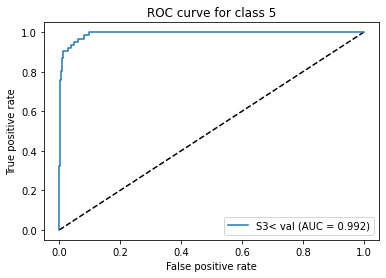
\includegraphics[width=0.7\textwidth]{3ROC5.png} %插入图片,[]中设置图片大小,{}中是图片文件名
    \caption{AUC for class 5:  0.9920098112085625} %最终文档中希望显示的图片标题
    \label{Fig.3ROC5} %用于文内引用的标签
\end{figure}
This is class 6\ref{Fig.ROC6}:
\begin{figure}[H] 
    \centering %图片居中
    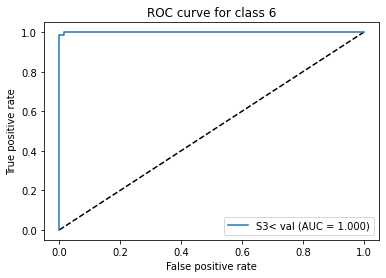
\includegraphics[width=0.7\textwidth]{3ROC6.png} %插入图片,[]中设置图片大小,{}中是图片文件名
    \caption{AUC for class 6:  0.9997770179872156} %最终文档中希望显示的图片标题
    \label{Fig.3ROC6} %用于文内引用的标签
\end{figure}
This is class 7\ref{Fig.ROC7}:
\begin{figure}[H] 
    \centering %图片居中
    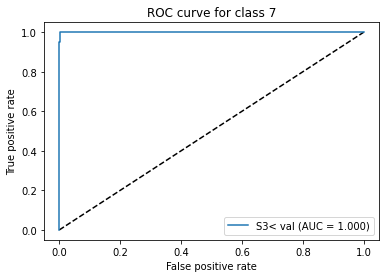
\includegraphics[width=0.7\textwidth]{3ROC7.png} %插入图片,[]中设置图片大小,{}中是图片文件名
    \caption{AUC for class 7:  0.9998885089936078} %最终文档中希望显示的图片标题
    \label{Fig.3ROC7} %用于文内引用的标签
\end{figure}
\subsubsection{normalized confusion matrix}
In this part, we discuss the normalized confusion matrix plot.Here is the code:
\begin{lstlisting}
    cm=confusion_matrix(list(y_test),list(y_predicted))
    cm_normalized = cm.astype('float') / cm.sum(axis=1)[:, np.newaxis]
    fig, ax = plt.subplots()
    im = ax.imshow(cm, interpolation='nearest', cmap=plt.cm.Blues)
    ax.figure.colorbar(im, ax=ax)
    classes=[0,1,2,3,4,5,6,7]
    # print(classes)
    # We want to show all ticks...
    ax.set(xticks=np.arange(cm_normalized.shape[1]),
        yticks=np.arange(cm_normalized.shape[0]),
        # ... and label them with the respective list entries
        xticklabels=classes, yticklabels=classes,
        ylabel='True label',
        xlabel='Predicted label')
    plt.setp(ax.get_xticklabels(),  ha="right",
                rotation_mode="anchor")
    thresh = cm_normalized.max() / 2.
    for i in range(cm_normalized.shape[0]):
        for j in range(cm_normalized.shape[1]):
            ax.text(j, i, format(cm_normalized[i, j], '.2f'),
                    ha="center", va="center",
                    color="white" if cm_normalized[i, j] > thresh else "black")
    fig.tight_layout()
\end{lstlisting}
The result plot is shown in Fig.\ref{Fig.t3q1c}.
\begin{figure}[H] 
    \centering %图片居中
    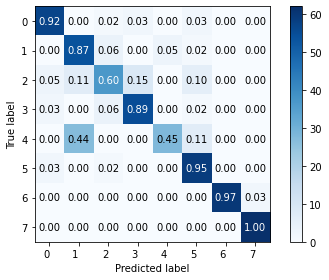
\includegraphics[width=0.7\textwidth]{T3Q1c.png} %插入图片,[]中设置图片大小,{}中是图片文件名
    \caption{normalized confusion matrix plot} %最终文档中希望显示的图片标题
    \label{Fig.t3q1c} %用于文内引用的标签
\end{figure}

\subsubsection{Precision, Recall, and F-1 score}
In this part, we discuss the normalized confusion matrix plot.Here is the code:
\begin{lstlisting}
    print(classification_report(y_true=y_test,y_pred=y_predicted))
\end{lstlisting}
The result plot is shown in Fig.\ref{Fig.t3q1d}.
\begin{figure}[H] 
    \centering %图片居中
    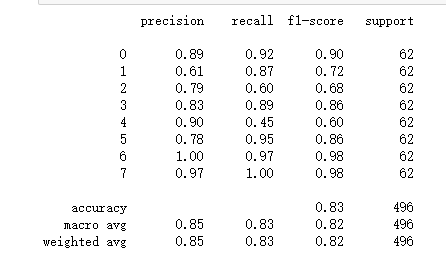
\includegraphics[width=0.7\textwidth]{T3Q1d.png} %插入图片,[]中设置图片大小,{}中是图片文件名
    \caption{Precision, Recall, and F-1 score} %最终文档中希望显示的图片标题
    \label{Fig.t3q1d} %用于文内引用的标签
\end{figure}

\subsection{Question 2}
方法用到HMT

CAPTUM可选项

\section{Task 4: Quantitative evaluation of the attribution methods}
应用,k设置为30,计算平均drop increase,HMT设置为90

讨论之前用过的方法,你的方法又没有正确反映特征,什么时候会失败,比较一下,给个reason


\begin{thebibliography}{00}
\bibitem{b1}Y. Gilad, R. Hemo, S. Micali, G. Vlachos, and N. Zeldovich, “Algorand: Scaling Byzantine Agreements for Cryptocurrencies,” in Proceedings of the 26th Symposium on operating systems principles, 2017, pp. 51–68. doi: 10.1145/3132747.3132757.
\bibitem{b2} King, Sunny, and Scott Nadal. "Ppcoin: Peer-to-peer crypto-currency with proof-of-stake." self-published paper, August 19.1, 2012.

\end{thebibliography}

\end{document}
